\documentclass{beamer}
\usepackage[latin1]{inputenc}
\usepackage{times}
\usepackage{tikz}
\usetheme{Luebeck}
%\usecolortheme{albatross}
\usepackage{amsmath,amsfonts,amsthm,amssymb}
\usepackage{setspace}
\usepackage{Tabbing}
\usepackage{fancyhdr}
\usepackage{lastpage}
\usepackage{extramarks}
\usepackage{chngpage}
\usepackage{soul,color}
\usepackage{graphicx,float,wrapfig}
\usepackage{xcolor}
\usepackage{listings}
\usepackage{float}
%\usepackage{subfloat}
\usepackage{subfigure}
\usepackage{caption}
\usepackage{enumitem}
\usepackage{algpseudocode}

\definecolor{darkorange}{RGB}{240, 120, 0}
\definecolor{darkgreen}{RGB}{0, 128, 0}

\setbeamercolor{background canvas}{bg=white}
\setbeamercolor{frametitle}{fg=white, bg=darkorange}
\setbeamercolor{normal text}{bg=black,fg=black}
\setbeamercolor{structure}{bg=black, fg=darkorange}


\lstdefinestyle{customc}{
  belowcaptionskip=1\baselineskip,
  breaklines=true,
  frame=L,
  xleftmargin=\parindent,
  language=Python,
  showstringspaces=false,
  basicstyle=\footnotesize\ttfamily,
  keywordstyle=\bfseries\color{green!40!black},
  commentstyle=\itshape\color{purple!40!black},
  identifierstyle=\color{blue},
  stringstyle=\color{orange},
}

\lstdefinestyle{customc}{
  belowcaptionskip=1\baselineskip,
  breaklines=true,
  frame=L,
  xleftmargin=\parindent,
  language=Python,
  showstringspaces=false,
  basicstyle=\footnotesize\ttfamily,
  keywordstyle=\bfseries\color{green!40!black},
  commentstyle=\itshape\color{purple!40!black},
  identifierstyle=\color{blue},
  stringstyle=\color{orange},
}

\lstdefinestyle{customcsmall}{
  belowcaptionskip=1\baselineskip,
  breaklines=true,
  frame=L,
  xleftmargin=\parindent,
  language=Python,
  showstringspaces=false,
  basicstyle=\footnotesize\ttfamily,
  keywordstyle=\bfseries\color{green!24!black},
  commentstyle=\itshape\color{purple!24!black},
  identifierstyle=\color{blue},
  stringstyle=\color{orange},
}

\lstdefinestyle{customcsmall}{
  belowcaptionskip=1\baselineskip,
  breaklines=true,
  frame=L,
  xleftmargin=\parindent,
  language=Python,
  showstringspaces=false,
  basicstyle=\footnotesize\ttfamily,
  keywordstyle=\bfseries\color{green!24!black},
  commentstyle=\itshape\color{purple!24!black},
  identifierstyle=\color{blue},
  stringstyle=\color{orange},
}

\definecolor{MidGreen}{HTML}{00AA00}
\definecolor{MidYellow}{HTML}{AAAA00}

\title{Lecture 19: Introduction To Topology}
\date{3/24/2016}
\institute{Chris Tralie, Duke University}
\author{COMPSCI/MATH 290-04}
\begin{document}

\frame{\titlepage}

\begin{frame}{Announcements}
\begin{itemize}[label=$\vartriangleright$]

\item Group Assignment 2 Due Wednesday 3/30

\item First project milestone Friday 4/8/2016

\item Welcome to unit 3!

\end{itemize}

\end{frame}

\begin{frame}{Table of Contents}
\begin{itemize}[label=$\blacktriangleright$]
	\item The Euler Characteristic
\end{itemize}
\begin{itemize}[label=$\vartriangleright$]
	\item Spherical Polytopes / Platonic Solids
\end{itemize}
\begin{itemize}[label=$\vartriangleright$]
	\item Fundamental Polygons, Tori
\end{itemize}
\begin{itemize}[label=$\vartriangleright$]
	\item Connected Sums, Genus
\end{itemize}
\end{frame}

\begin{frame}{Graphs Review}


\end{frame}


\begin{frame}{Planar Graphs}



\end{frame}


\begin{frame}{The Euler Characteristic}

\only<1-2>{
\[ \chi = V - E + F \]
}

\only<3> {
\[ \chi = V - E + F = 2 \]
}

\uncover<2->{
Planar graphs?
}




\end{frame}

\begin{frame}{The Euler Characteristic: Proof}



\end{frame}


\begin{frame}{Table of Contents}
\begin{itemize}[label=$\vartriangleright$]
	\item The Euler Characteristic
\end{itemize}
\begin{itemize}[label=$\blacktriangleright$]
	\item Spherical Polytopes / Platonic Solids
\end{itemize}
\begin{itemize}[label=$\vartriangleright$]
	\item Fundamental Polygons, Tori
\end{itemize}
\begin{itemize}[label=$\vartriangleright$]
	\item Connected Sums, Genus
\end{itemize}
\end{frame}

\begin{frame}{Regular Polygons}

\end{frame}

\begin{frame}{Stereographic Projection}

\begin{figure}[t]
    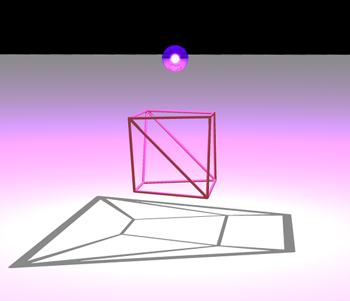
\includegraphics[width=0.6\textwidth]{shadow.png}
\end{figure}

\small \url{http://www.ics.uci.edu/~eppstein/junkyard/euler/}

\end{frame}


\begin{frame}{Regular Polyhedra (Platonic Solids)}

The Tetrahedron: 4 Vertices, 4 Faces, Triangle Faces

\begin{figure}[t]
    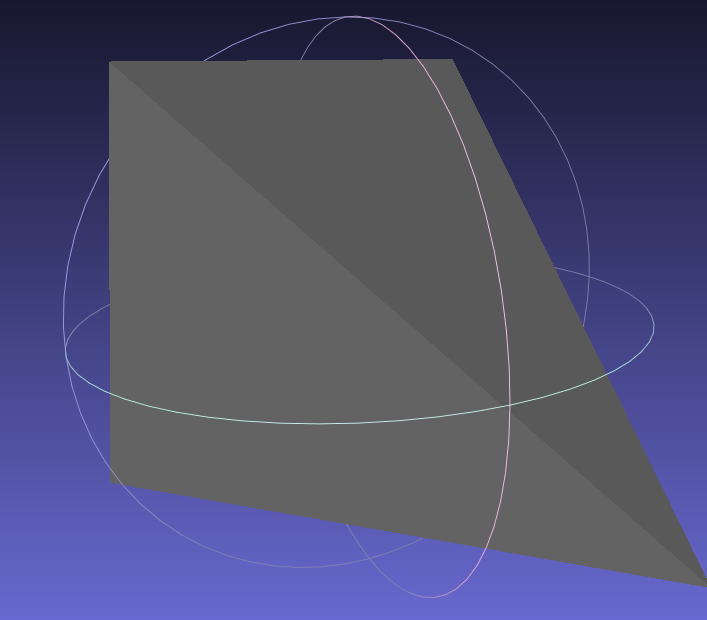
\includegraphics[width=0.6\textwidth]{PlatonicSolids/Tetrahedron.png}
\end{figure}

\end{frame}



\begin{frame}{Regular Polyhedra (Platonic Solids)}

The Cube: 8 Vertices, 6 Faces, Square Faces

\begin{figure}[t]
    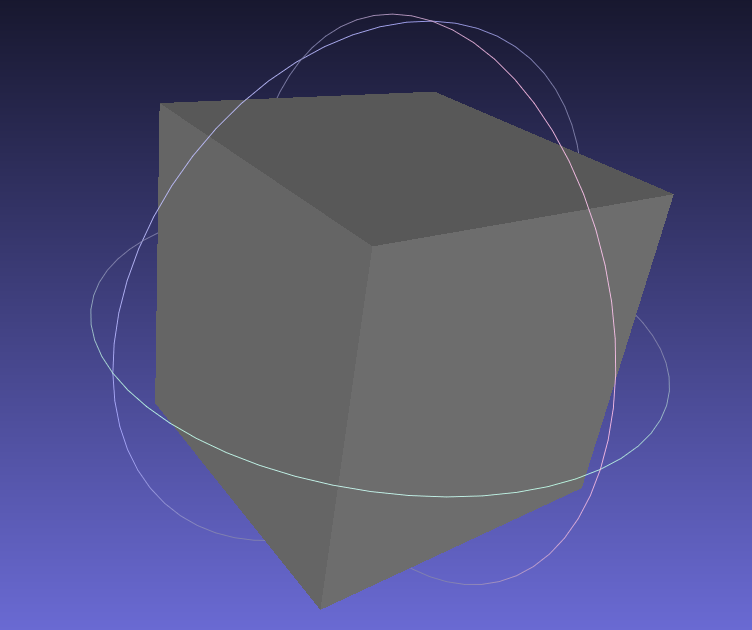
\includegraphics[width=0.6\textwidth]{PlatonicSolids/Cube.png}
\end{figure}

\end{frame}


\begin{frame}{Regular Polyhedra (Platonic Solids)}

The Octahedron: 6 Vertices, 8 Faces, Triangle Faces

\begin{figure}[t]
    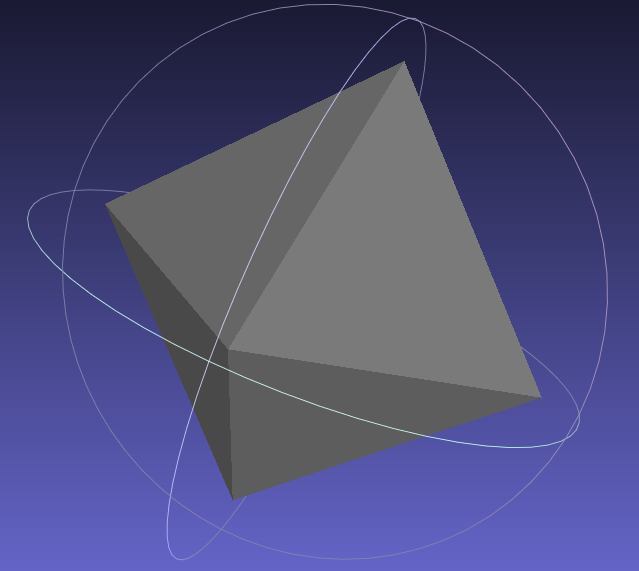
\includegraphics[width=0.6\textwidth]{PlatonicSolids/Octahedron.png}
\end{figure}

\end{frame}


\begin{frame}{Regular Polyhedra (Platonic Solids)}

The Dodecahedron: 20 Vertices, 12 Faces, Pentagonal Faces

\begin{figure}[t]
    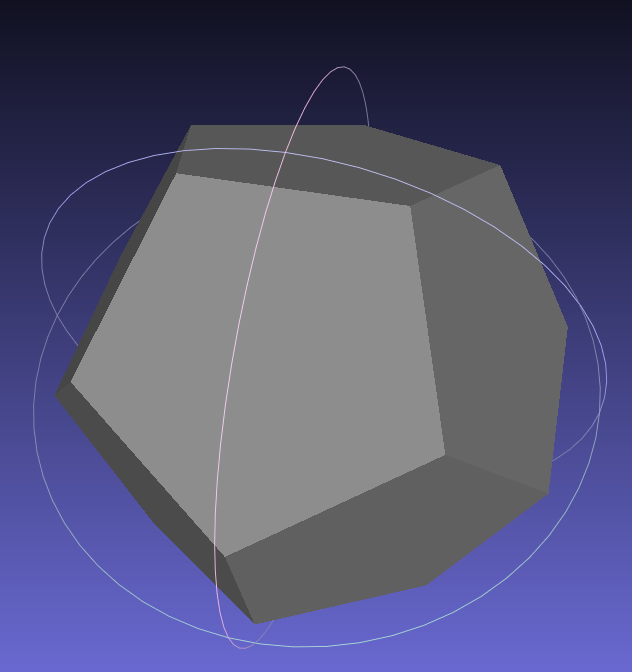
\includegraphics[width=0.6\textwidth]{PlatonicSolids/Dodecahedron.png}
\end{figure}

\end{frame}



\begin{frame}{Regular Polyhedra (Platonic Solids)}

The Icosahedron: 12 Vertices, 20 Faces, Triangle Faces

\begin{figure}[t]
    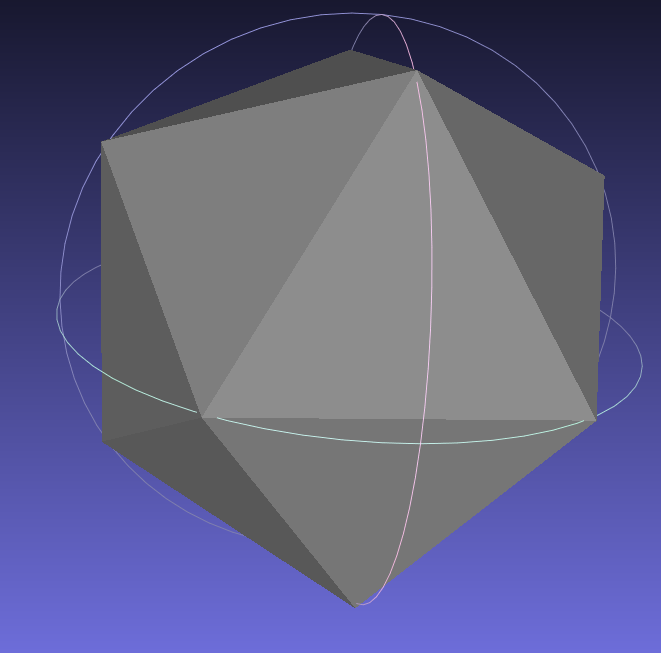
\includegraphics[width=0.6\textwidth]{PlatonicSolids/Icosahedron.png}
\end{figure}

\end{frame}


\begin{frame}{Constructing The Tetrahedron}

\begin{figure}[t]
    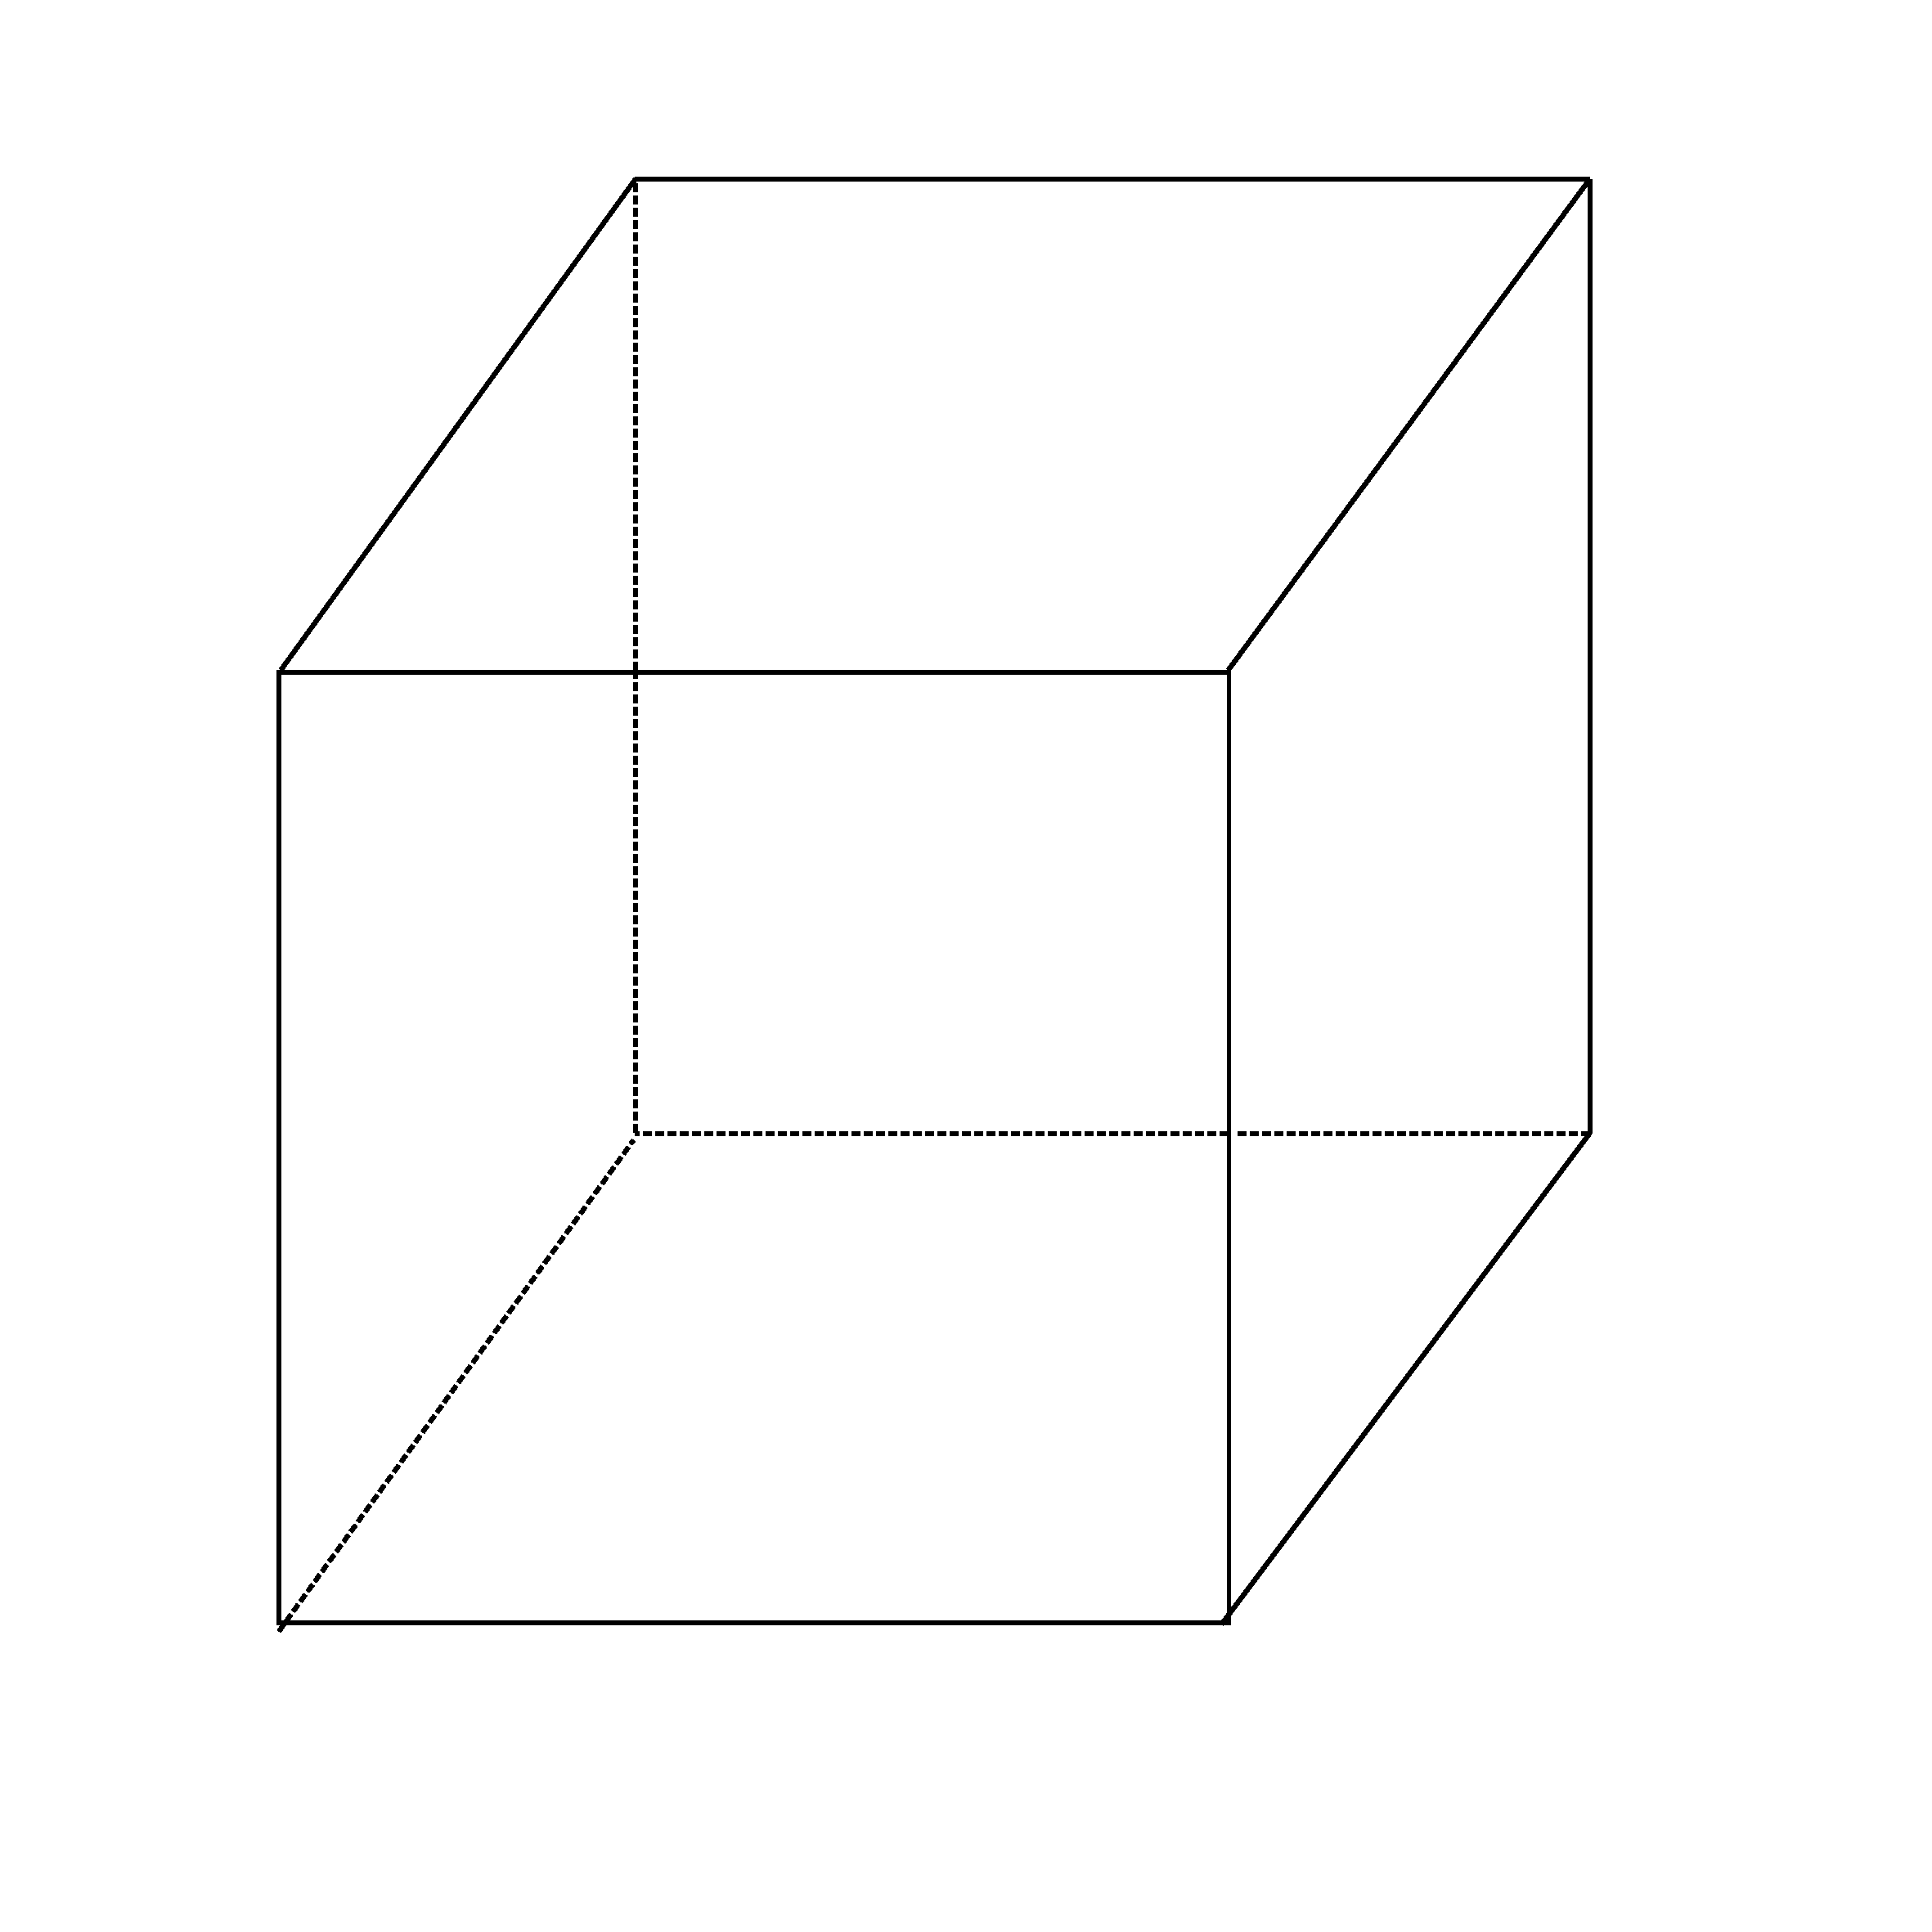
\includegraphics[width=0.6\textwidth]{CubeConstruct.pdf}
\end{figure}

\end{frame}


\begin{frame}{Constructing The Icosahedron}

\begin{figure}[t]
    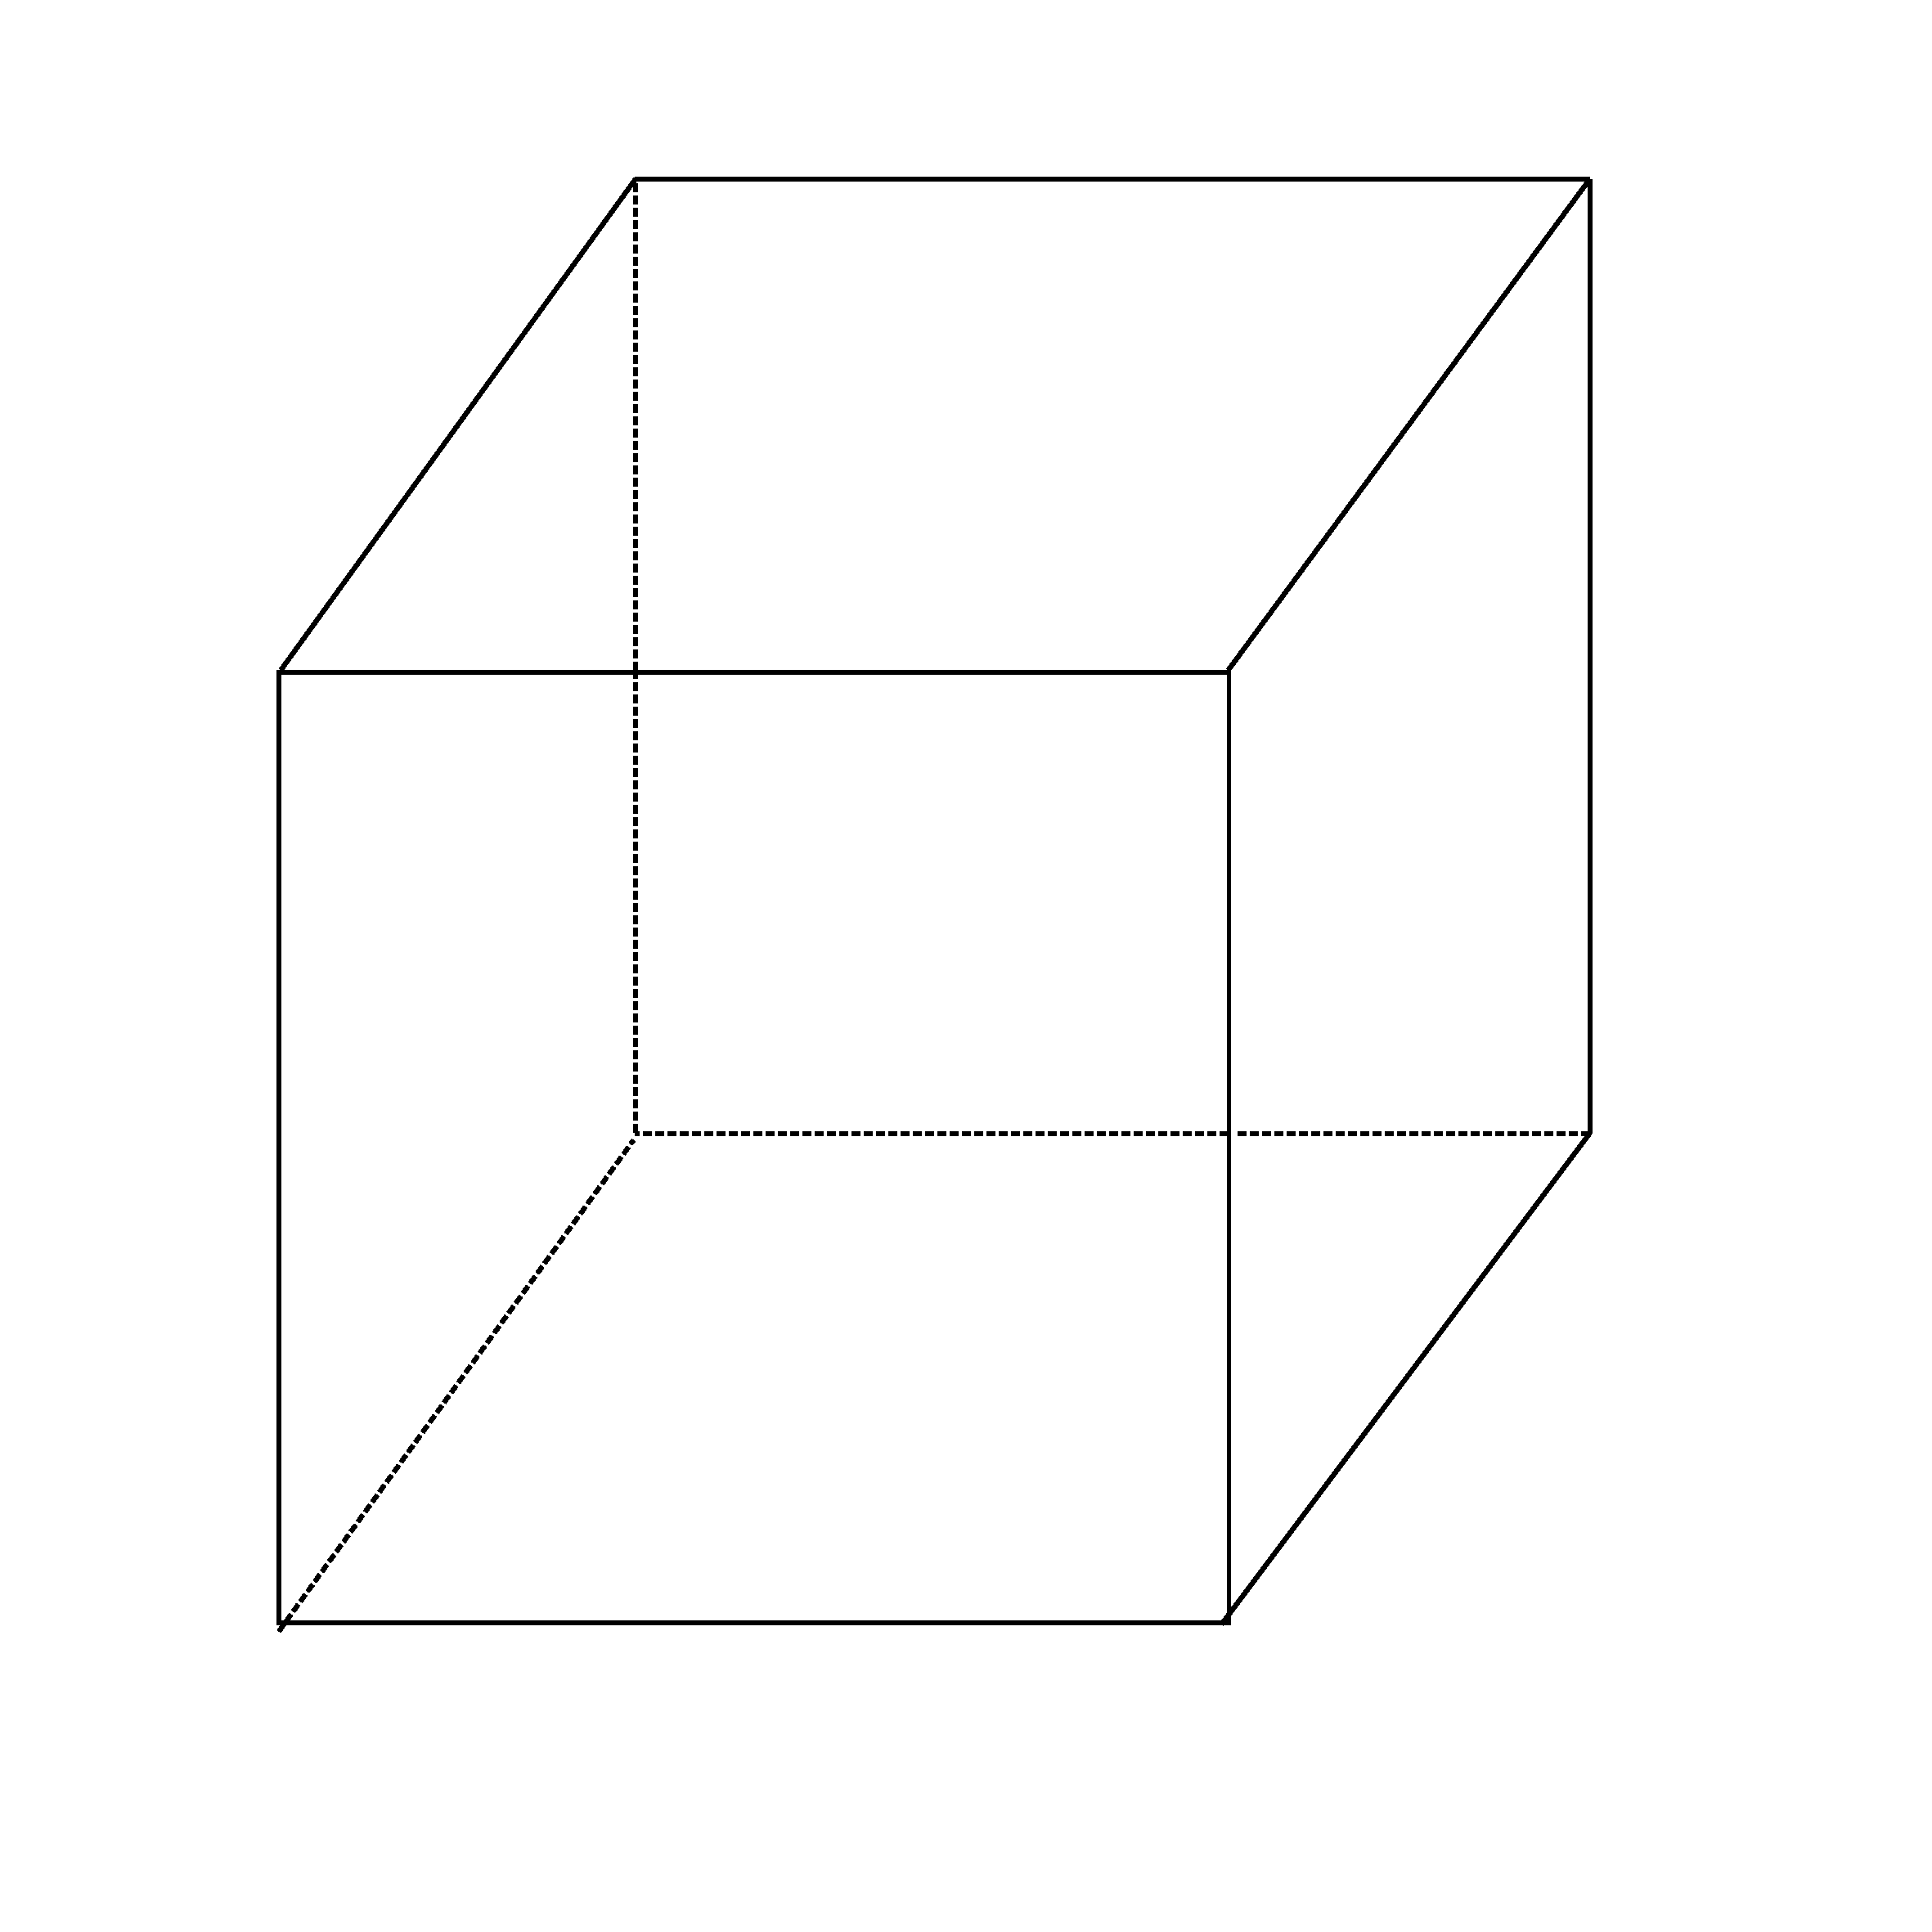
\includegraphics[width=0.6\textwidth]{CubeConstruct.pdf}
\end{figure}

\end{frame}

\begin{frame}{Platonic Solids: Is This it??}

Let $p$ be the number of sides per face, $q$ be the {\em degree} of each vertex

\uncover<2->{
\[ pF = 2E = qV \]
}

\uncover<3->{

Combine with $V - E + F = 2$

\[ \frac{2E}{q} - E + \frac{2E}{p} = 2 \]

}

\uncover<4->{

\[  \frac{1}{q} + \frac{1}{p} = \frac{1}{2} + \frac{1}{E} \]

}

\uncover<5->{

\[ \implies \frac{1}{q} + \frac{1}{p} > \frac{1}{2} \]

}

\end{frame}



\begin{frame}{Flattening To Plane}

We don't need convex polygons, as long as they are ``sphere-like''

\uncover<2->{
\begin{figure}[t]
    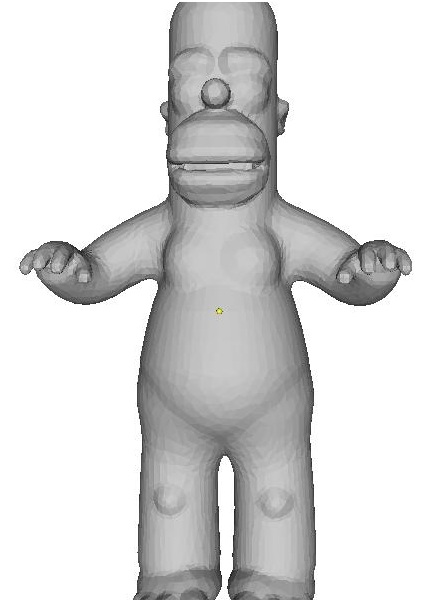
\includegraphics[width=0.5\textwidth]{homerparam1.jpg}
\end{figure}
}

\end{frame}

\begin{frame}{Flattening To Plane}

\begin{figure}[t]
    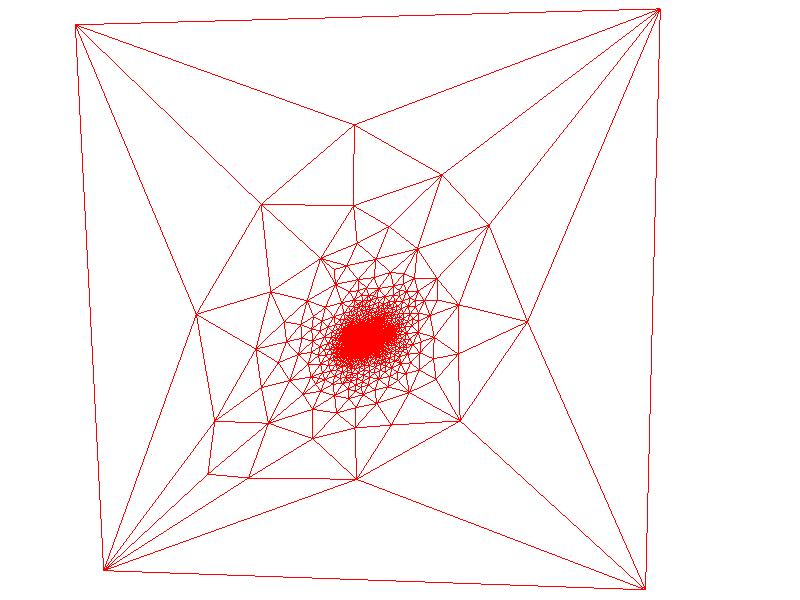
\includegraphics[width=0.8\textwidth]{homerparam2.jpg}
\end{figure}

\end{frame}

\begin{frame}{Flattening To Plane}

\begin{figure}[t]
    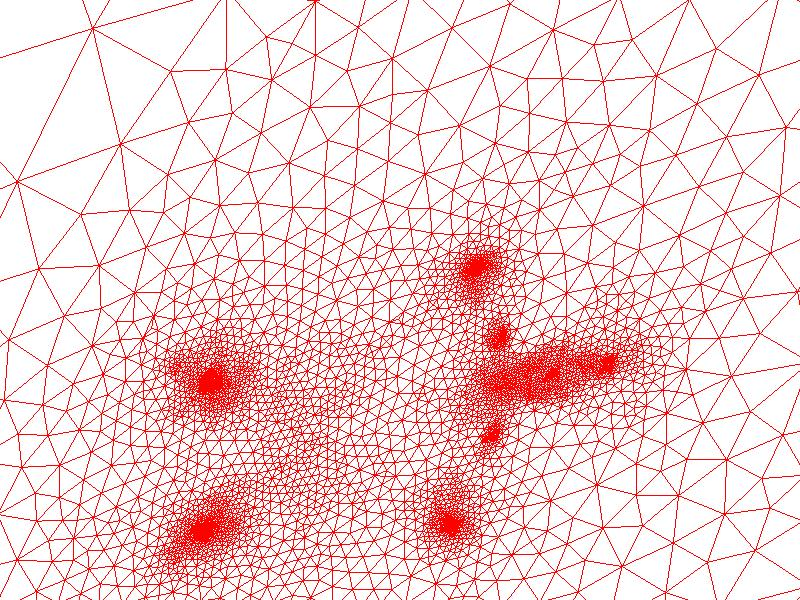
\includegraphics[width=0.8\textwidth]{homerparam3.jpg}
\end{figure}

\end{frame}

\begin{frame}{Flattening To Plane}

\begin{figure}[t]
    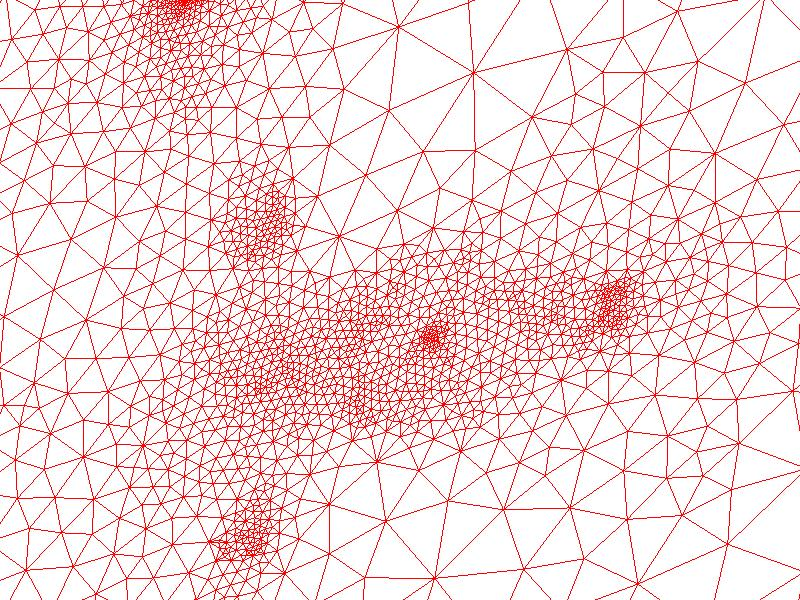
\includegraphics[width=0.8\textwidth]{homerparam4.jpg}
\end{figure}

\end{frame}

\begin{frame}{Table of Contents}
\begin{itemize}[label=$\vartriangleright$]
	\item The Euler Characteristic
\end{itemize}
\begin{itemize}[label=$\vartriangleright$]
	\item Spherical Polytopes / Platonic Solids
\end{itemize}
\begin{itemize}[label=$\blacktriangleright$]
	\item Fundamental Polygons, Tori
\end{itemize}
\begin{itemize}[label=$\vartriangleright$]
	\item Connected Sums, Genus
\end{itemize}
\end{frame}


\begin{frame}{The Torus}

\begin{figure}[t]
    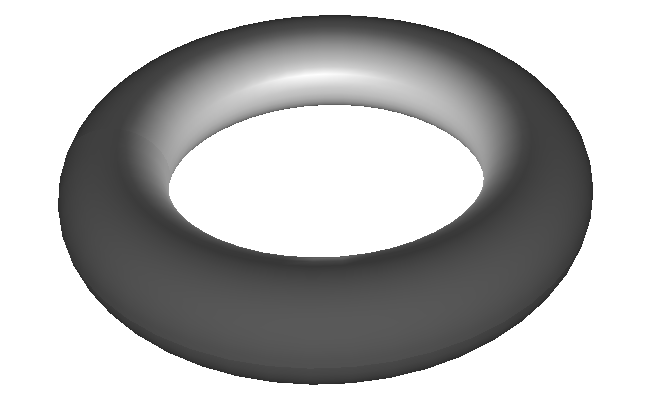
\includegraphics[width=0.7\textwidth]{TorusFull.png}
\end{figure}

\end{frame}


\begin{frame}{Constructing Torus}

Show Video

\end{frame}

\begin{frame}{Torus Fundamental Polygon}

\uncover<2->{

\begin{itemize}[label=$\blacktriangleright$]
\item What is the Euler characteristic of a torus?
\end{itemize}

}

\begin{figure}[t]
    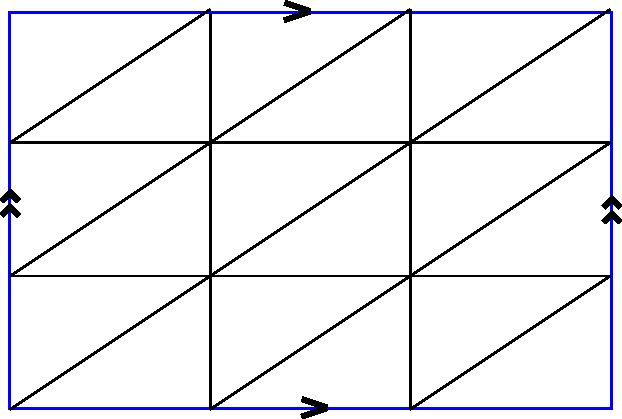
\includegraphics[width=0.8\textwidth]{FundamentalPolygon.pdf}
\end{figure}

\end{frame}


\begin{frame}{Intermezzo: Rhythm And Tori / Grateful Dead}



\end{frame}


\begin{frame}{Table of Contents}
\begin{itemize}[label=$\vartriangleright$]
	\item The Euler Characteristic
\end{itemize}
\begin{itemize}[label=$\vartriangleright$]
	\item Spherical Polytopes / Platonic Solids
\end{itemize}
\begin{itemize}[label=$\vartriangleright$]
	\item Fundamental Polygons, Tori
\end{itemize}
\begin{itemize}[label=$\blacktriangleright$]
	\item Connected Sums, Genus
\end{itemize}
\end{frame}


\begin{frame}{Duplicating Spheres}

What's the euler characteristic of two spheres?

\begin{figure}[t]
    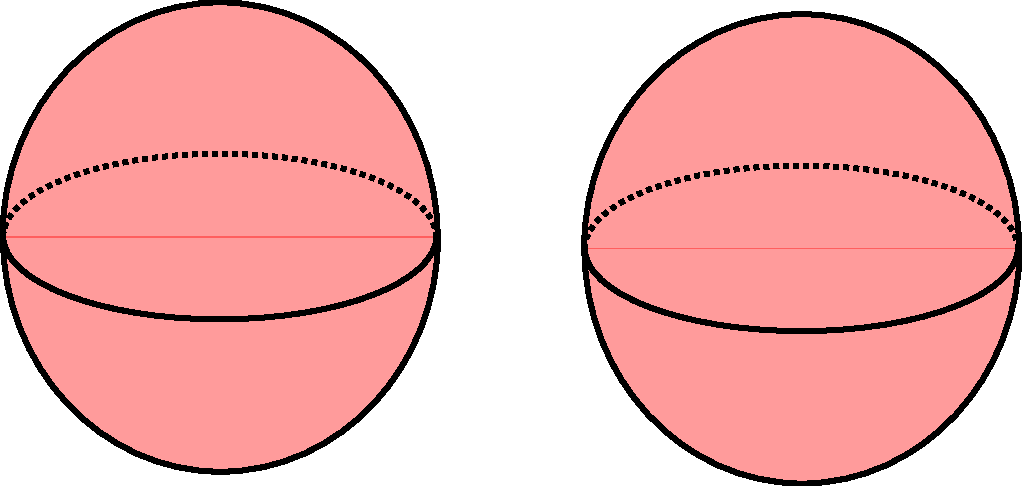
\includegraphics[width=\textwidth]{2Spheres.pdf}
\end{figure}


\end{frame}


\begin{frame}{Duplicating Tori}

What's the euler characteristic of two tori?

\begin{figure}[t]
    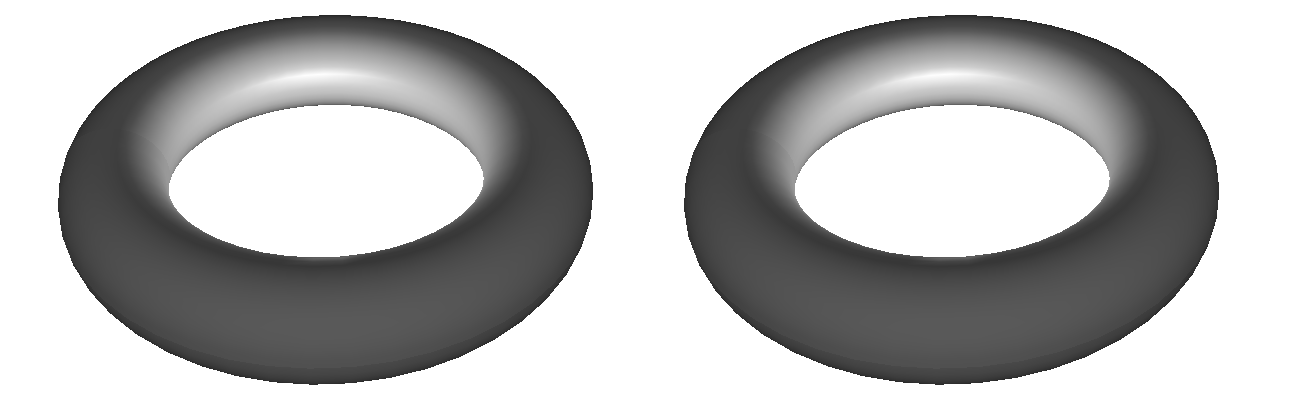
\includegraphics[width=\textwidth]{2Tori.png}
\end{figure}

\end{frame}

\begin{frame}{Connected Sum}

$T_1 \# T_1 = T_2$

\begin{figure}[t]
    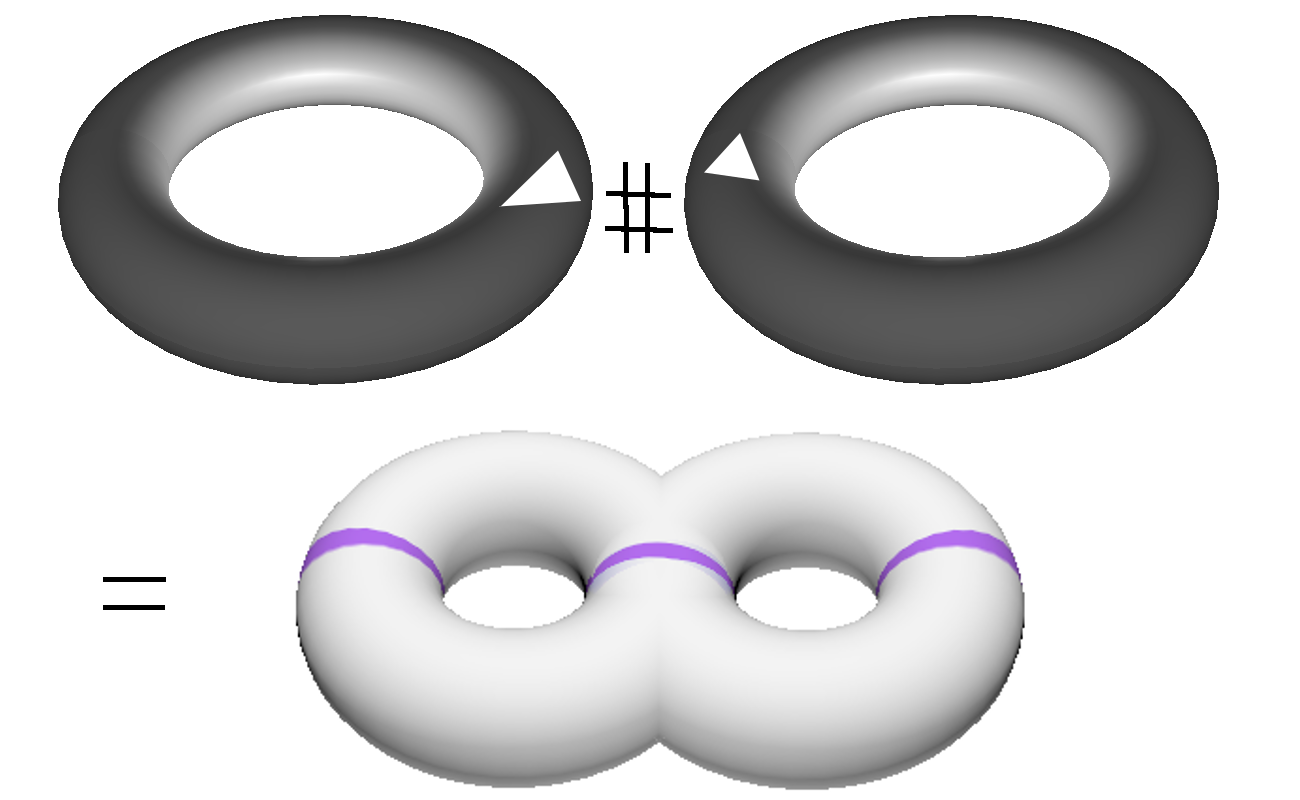
\includegraphics[width=\textwidth]{ConnectedSum.png}
\end{figure}

\end{frame}


\begin{frame}{Connected Sum}

$T_1 \# T_1 = T_2$

What is the Euler characteristic?

\begin{figure}[t]
    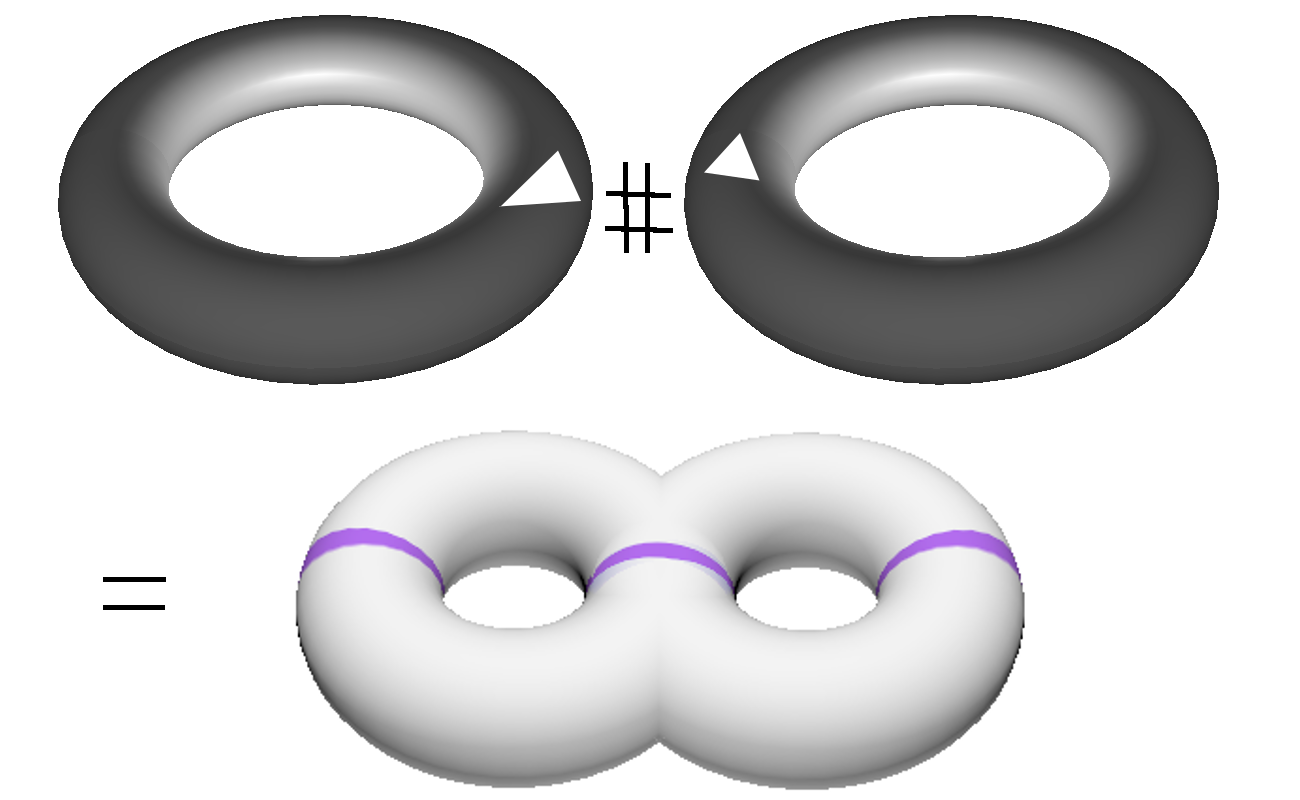
\includegraphics[width=0.6\textwidth]{ConnectedSum.png}
\end{figure}

\end{frame}


\begin{frame}{Connected Sum: g Tori}

What is the Euler characteristic of $T_N = T_1 \# T_1 \# \hdots \# T_1$ g times?

\uncover<2->{

\[ \chi = 2 - 2g \]


}

\uncover<3->{
\begin{itemize}[label=$\blacktriangleright$]

    \item $g$ is known as the ``genus''

\end{itemize}
}

\end{frame}

\begin{frame}{Connected Sum with Spheres}

What is the connected sum of a sphere with a sphere?

\end{frame}

\begin{frame}{Connected Sum with Spheres}

What is the connected sum of a torus with a sphere?

\end{frame}


\begin{frame}{Euler Characteristic: Homology}

\[ \chi = \beta_0 - \beta_1 + \beta_2 \]

\begin{itemize}[label=$\blacktriangleright$]

\item $\beta_0$: Number of connected components

\item $\beta_1$: Number of independent loops/cycles

\item $\beta_2$ Number of independent voids

\end{itemize}

\end{frame}

\end{document}

